\documentclass[10pt]{article}
\usepackage[margin=0.8in]{geometry}
\usepackage{amsmath,amssymb,amsthm,booktabs,tabularx,array,hyperref,microtype,graphicx,needspace}
\emergencystretch=1.5em
\hypersetup{colorlinks=true,linkcolor=blue,urlcolor=blue,citecolor=blue,pdftitle={Brake, Switch, Stay Safe: A Lean Proof for an Actuator with Uncertain Lag}}
\newtheorem{theorem}{Theorem}
\newcommand{\R}{\mathbb R}
\newcommand{\E}{\mathcal E}
\newcommand{\clip}{\operatorname{clip}}
\newcommand{\code}[1]{\texttt{#1}}
\title{Brake, Switch, Stay Safe\\\large A Lean Proof for an Actuator with Uncertain Lag}
\author{Mike\\\small Working draft; full author details and affiliation pending}
\date{17 October 2026}
\begin{document}
\maketitle
\begin{abstract}
An invariant-set theorem gives no guarantee for a system that starts outside its admitted region. We prove a recovery maneuver for an actuator with uncertain fixed lag. A held braking command keeps position within its limits and reaches a certified ellipsoid. The controller then switches to sampled saturated feedback without a state reset. The entire initial box lies outside the ellipsoid. Lean checks the path, terminal energy, continuous handoff, and execution existence and uniqueness. The proof covers every admitted initial state and lag rate. A second theorem gives the result in physical units. Direct feedback also succeeds in our numerical tests. A stronger rational interval prototype covers the whole initial box. A reusable Lean checker now proves endpoint containment and terminal entry for one direct-feedback subbox; the full direct-feedback safety proof remains open. The evidence supports a reproducible verification case study. It does not establish better control performance or a new recovery method.
\end{abstract}

\section{The problem and the exact claim}
A stopping calculation does not establish two-sided position safety when acceleration has its own dynamics. At zero velocity, nonzero acceleration can drive the axis toward the opposite limit. A recovery proof must cover the entire motion before the switch. It must also connect the terminal state to a controller with a certified future behavior.

\begin{figure}[tbp]
\centering
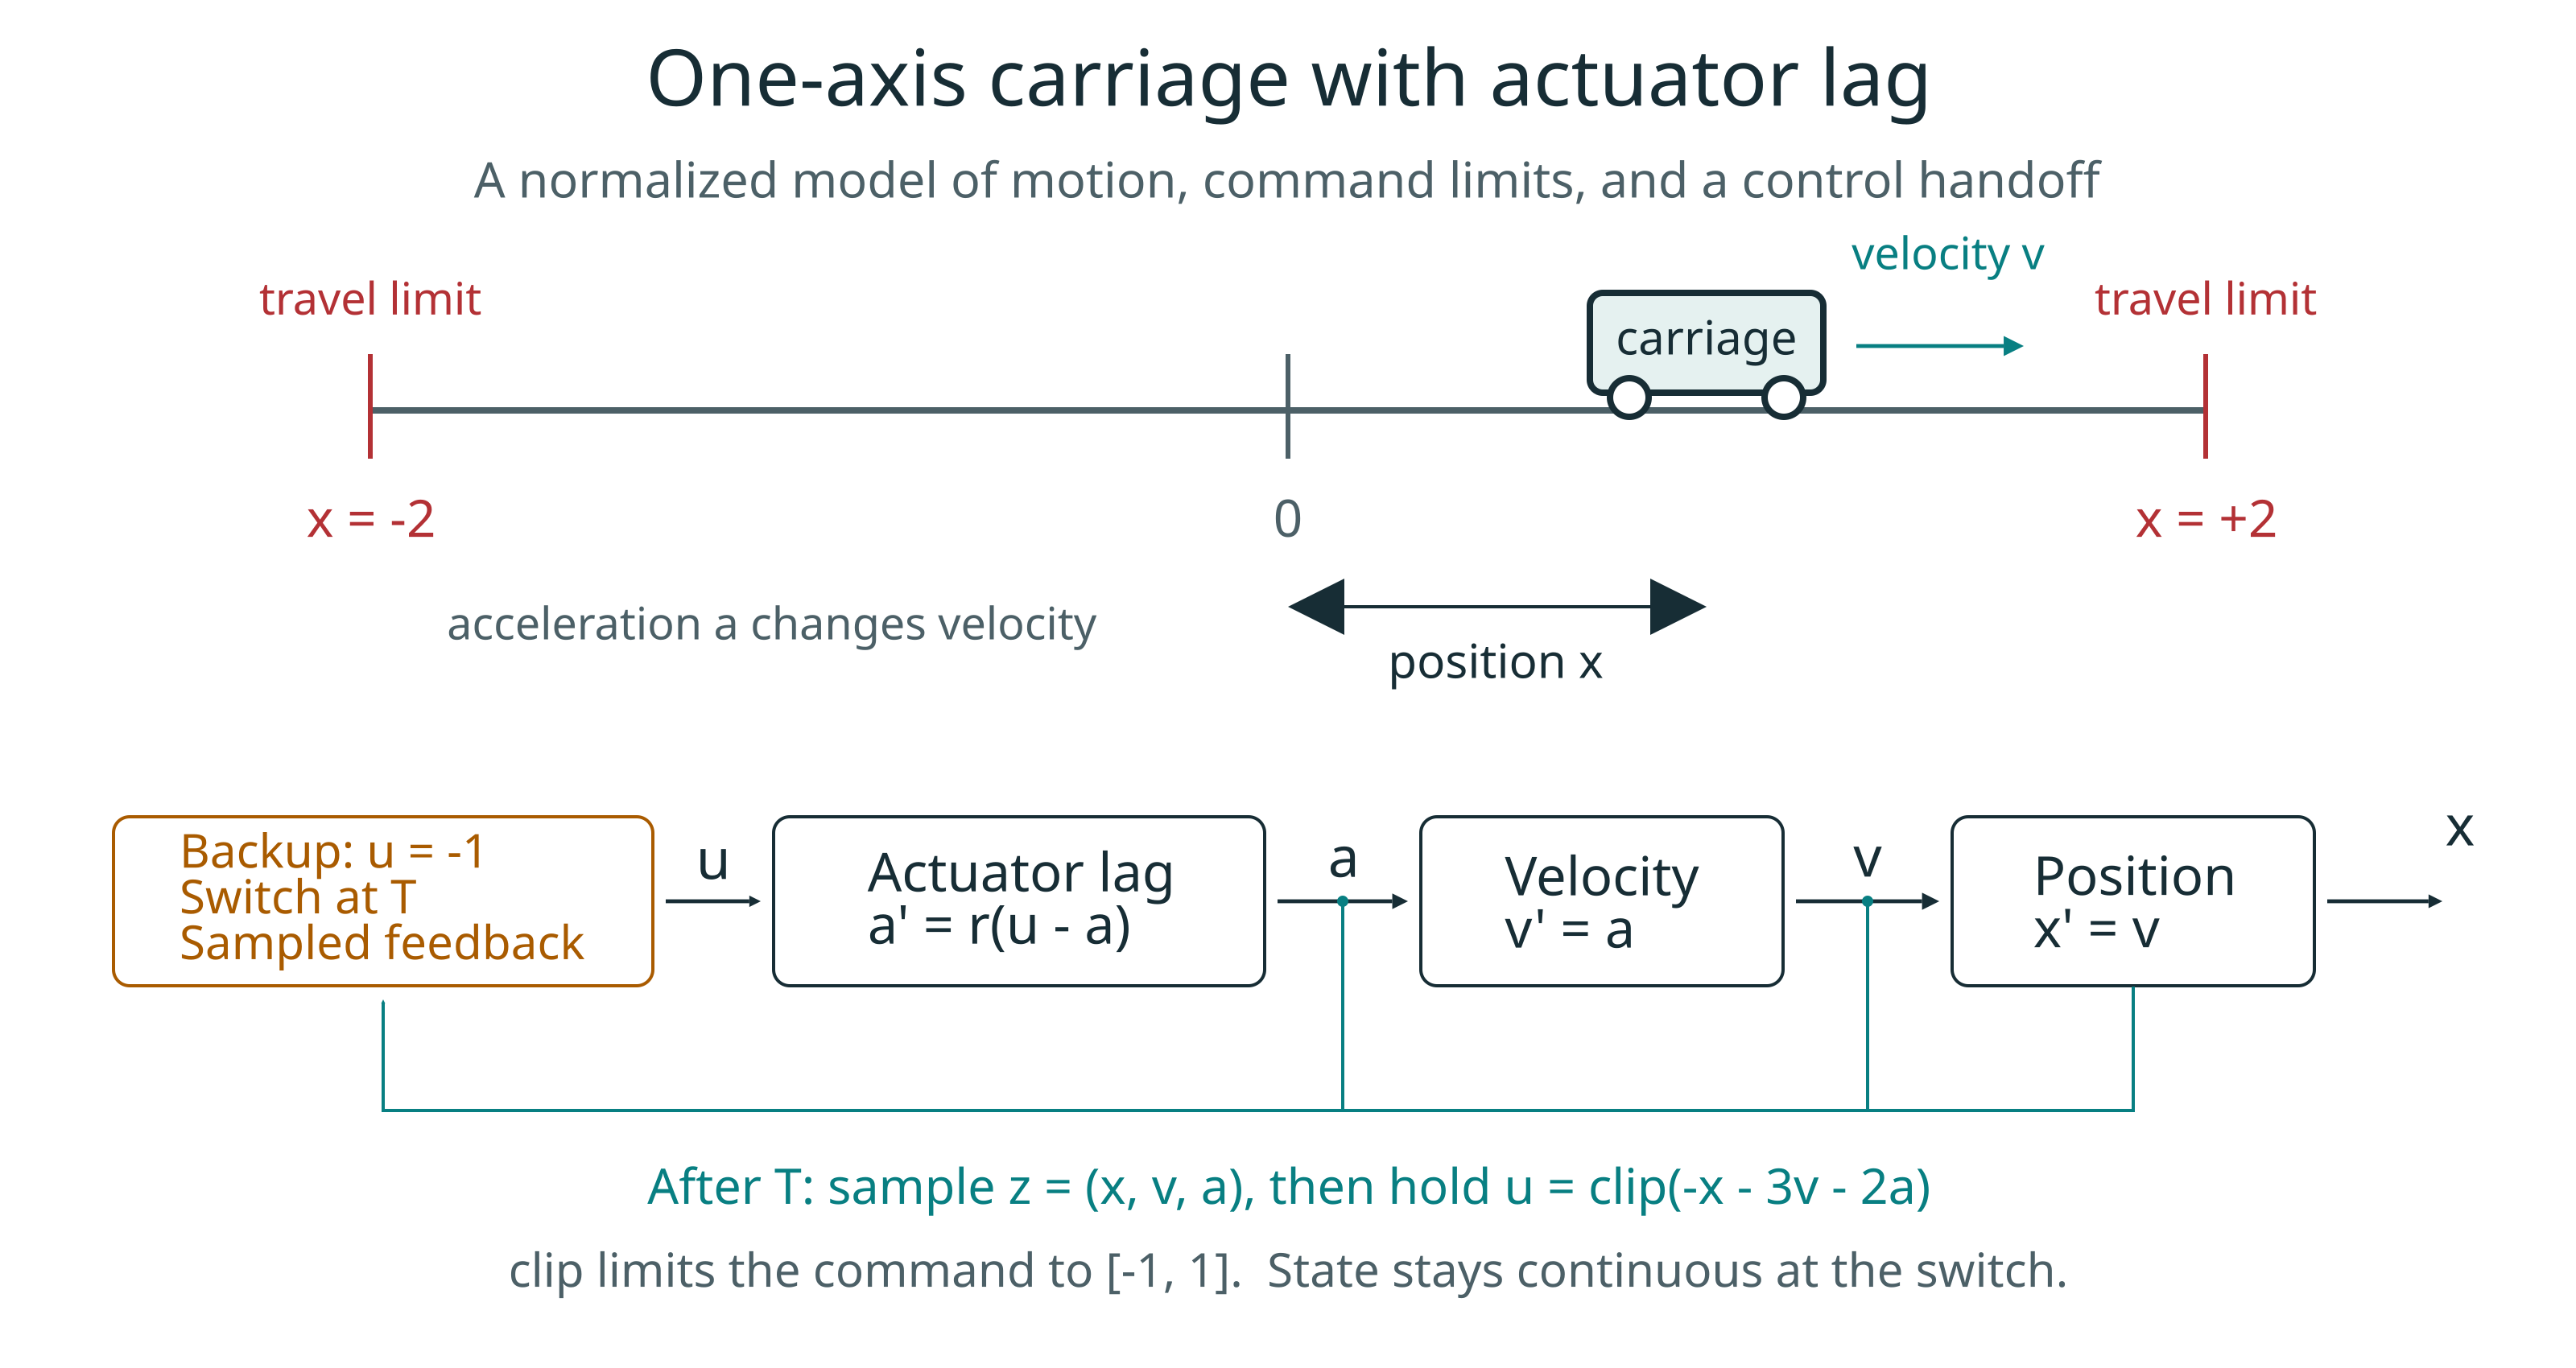
\includegraphics[width=\textwidth]{images/carriage-model.png}
\caption{An ideal carriage on a straight rail. The command passes through actuator lag before it changes acceleration. The sampled controller receives the state tuple $(x,v,a)$. This diagram shows the zero-error case. Travel limits are model constraints; the diagram does not represent calibrated hardware or physical stops.}
\label{fig:carriage}
\end{figure}

We study the normalized plant
\begin{equation}\label{eq:plant}
\dot x=v,\qquad \dot v=a,\qquad \dot a=r(u-a),
\end{equation}
with one unknown but fixed rate $r\in[9/10,11/10]$. The position requirement is $|x(t)|\le2$. It is not a bound on accumulated distance, and the plant includes no contact or collision model.

Our maneuver holds $u=-1$ until $T=5/4$. At $T$, it starts a new sampling clock and uses
\begin{equation}\label{eq:control}
k(z)=-x-3v-2a,\qquad
u_n=\clip_{[-1,1]}(k(f(T+t_n))+e_n)+d_n.
\end{equation}
Here $t_0=0$, $t_{n+1}=t_n+h_n$, and $e_n,d_n$ are held constant on each interval. The drive error enters inside the multiplier $r$. Thus the actual drive can exceed the clamp limit by $|d_n|$. There are no command errors or disturbances during the initial brake.

The starting box is
\begin{equation}\label{eq:box}
\mathcal B=
[99/100,101/100]\times[49/100,51/100]\times[-1/100,1/100].
\end{equation}
Define $\E(z)=z^\top Pz$, written $V$ in the Lean code and figures, with
\begin{equation}\label{eq:P}
P=\begin{pmatrix}
38/5&257/25&5\\
257/25&1319/50&769/50\\
5&769/50&278/25
\end{pmatrix},\qquad
\mathcal S=\{z:\E(z)\le12\}.
\end{equation}
A prior part of the same local artifact certifies $\mathcal S$ for the sampled controller. The present extension supplies a safe path into $\mathcal S$.

\Needspace{14\baselineskip}
\begin{theorem}[Concrete recovery and continuous handoff]\label{thm:main}
Let $z_0\in\mathcal B$ and $r\in[9/10,11/10]$. Suppose some $h_{\min}>0$ satisfies
\[
h_{\min}\le h_n\le1/5,\qquad |e_n|+|d_n|\le1/90
\]
for every $n$. There exists a continuous execution of \eqref{eq:plant} that starts at $z_0$, holds $u=-1$ on $(0,T)$, and obeys \eqref{eq:control} on every $(T+t_n,T+t_{n+1})$. Any two such executions for the same prescribed parameters and error sequences agree for all $t\ge0$. Every such execution satisfies
\[
|x(t)|\le2\quad(t\ge0),\qquad \E(f(T))\le12.
\]
Every admitted starting state is outside the old ellipsoid:
\[
\E(z_0)\ge11749189/500000=23.498378>12.
\]
\end{theorem}

The execution contract requires continuity of all three coordinates. Its feedback uses the trajectory's own sampled state. The theorem derives agreement with the analytic solution and terminal safety. It does not assume either property. Derivatives need exist only inside the open hold intervals. The rate stays fixed before and after the switch.

Taken together, the two safety contracts support the mathematical design of a one-time choice: direct operation inside $\mathcal S$ or recovery inside $\mathcal B$. The implementation of that initial-state selector is not formalized here. We do not prove repeated switching or a general runtime shield that accepts arbitrary requested inputs.

\section{Proof of the recovery transient}
For a fixed held input, \eqref{eq:plant} has the solution
\begin{align}
a(s)&=u+(a_0-u)e^{-rs},\nonumber\\
v(s)&=v_0+us+(a_0-u)(1-e^{-rs})/r,\label{eq:flow}\\
x(s)&=x_0+v_0s+us^2/2+
(a_0-u)\bigl(s/r-(1-e^{-rs})/r^2\bigr).\nonumber
\end{align}
The existing artifact checks initial values and all three derivatives. Uniqueness on a closed hold follows by multiplying an acceleration difference by $e^{rs}$, applying a mean-value argument, then applying the same argument to velocity and position differences. Continuity includes the endpoints.

\subsection{All-time travel during the long brake}
For $u=-1$, $r>0$ and $s\ge0$, the initial acceleration interval gives
\[
-1\le a(s)\le1/100.
\]
Two derivative-comparison arguments establish
\[
x_0+v_0s-s^2/2\le x(s)
\le x_0+v_0s+s^2/200.
\]
On $0\le s\le5/4$, the initial box then implies the checked rational bounds
\begin{equation}\label{eq:path}
657/800\le x(s)\le5297/3200.
\end{equation}
Both endpoints lie strictly inside $[-2,2]$. The upper polynomial is increasing; the lower concave polynomial is bounded below by its endpoint minimum. This proof is independent of the sampled controller's maximum hold length. In particular, we never apply its $1/5$-time certificate to the $5/4$-time brake.

\subsection{Terminal entry by a checked finite covering}
Substituting $T=5/4$ into \eqref{eq:flow} leaves one transcendental term, $e^{-5r/4}$. We divide $[9/10,11/10]$ into 32 closed intervals, each of width $1/160$. This is a covering of every real rate, not evaluation on a grid.

At each of the 33 endpoints, set $q=-5r/4$ and approximate $\exp(q/2)$ by its degree-nine Taylor polynomial. The existing mathlib bound applies because $|q/2|\le11/16<1$:
\[
\left|\exp(q/2)-\sum_{m=0}^{9}\frac{(q/2)^m}{m!}\right|
\le |q/2|^{10}\frac{11}{10!\,10}.
\]
The producer rounds these bounds outward to rational numbers. Lean checks the resulting inequalities, uses positive squaring to obtain bounds for $\exp(q)$, and uses exponential monotonicity within each rate interval. Positive reciprocal bounds enclose $1/r$.

Cancellation in $\E$ matters. A direct interval evaluation of its expanded cross terms is unnecessarily wide. Instead, Lean verifies the exact identity
\begin{align}
\E(z)={}&\frac{38}{5}\left(x+\frac{257}{190}v+\frac{25}{38}a\right)^2
+\frac{29628}{2375}\left(v+\frac{20465}{29628}a\right)^2\nonumber\\
&+\frac{1391479}{740700}a^2.\label{eq:ldl}
\end{align}
A non-native dyadic interval tactic checks this expression on each rate cell and on the entire initial box simultaneously. The endpoint flow is therefore certified to satisfy $\E\le12$ for every allowed rate and initial state. This proof does not need the separate eight-corner convexity argument used in the exploratory Python diagnostic.

The earlier diagnostic obtained an upper bound near $11.2344$ using a different, finer covering. That number is not the bound exported by this Lean theorem. The formal terminal conclusion is $\E\le12$.

\section{Handoff to the sampled invariant}
The existing invariant proof uses the same $P$, controller and error placement. It establishes $x^2\le\E(z)/3$, so $\mathcal S$ implies travel safety. Inside $\mathcal S$, the clipped feedback admits a sector gain in $[2/5,1]$. A shared exponential remainder and quadratic Bernstein representation in $r$ reduce the nominal held-flow inequality to twelve exact rational matrix certificates. They imply
\[
\E(z_{\rm nom}(s))\le\E(z_0)-\tfrac32s\|z_0\|_2^2,\qquad 0\le s\le1/5.
\]
The response to an additional held drive $w$ satisfies
$\E(g(r,s)w)\le16s^2w^2$. An elapsed-time-scaled Young inequality and the $1/90$ error budget preserve $\mathcal S$ throughout each hold. Sample induction and the positive dwell lower bound extend this guarantee to all nonnegative times.

The new handoff proof first derives
\[
f(s)=\operatorname{heldFlow}(r,s,z_0,-1)\quad(0\le s\le T)
\]
from the actual recovery ODE and continuity. It then defines $g(s)=f(T+s)$ and proves that $g$ satisfies the existing sampled execution contract, with initial value $f(T)$ and sampled feedback $g(t_n)$. The terminal certificate supplies $\E(f(T))\le12$.

For existence, an explicit piecewise trajectory uses the held solution through $T$ and the constructed sampled solution afterwards. Their full state values agree at $T$. The resulting trajectory is continuous and satisfies both ODE branches. Uniqueness uses held-flow uniqueness before the handoff and sampled-execution uniqueness afterwards. These existence arguments need no safety premise, ruling out a vacuous universal safety statement.

\section{Physical units and an illustrative axis}
Let $\tau_0>0$ be the nominal time constant used in the gains, $\tau>0$ the actual fixed lag, and $U>0$ the command scale. Normalize physical position, velocity, acceleration and time by
\[
z=\left(\frac{X}{U\tau_0^2},\frac{V}{U\tau_0},\frac{A}{U}\right),
\qquad t=\frac{s}{\tau_0},\qquad r=\frac{\tau_0}{\tau}.
\]
The physical plant is $\dot X=V$, $\dot V=A$, and
$\tau\dot A=u-A$. Brake with $u=-U$ until $s=5\tau_0/4$. Thereafter the held request is
$-X/\tau_0^2-3V/\tau_0-2A$, with clamp $[-U,U]$.

Lean proves normalization of an arbitrary physical recovery execution, including the derivatives and its own sampled feedback. If the normalized initial state belongs to $\mathcal B$, $\tau_0/\tau\in[.9,1.1]$, the physical holds lie in $[h_{\min},\tau_0/5]$ for some positive $h_{\min}$, and the post-handoff errors obey
$|\varepsilon_n|+|\Delta_n|\le U/90$, then
\[
|X(s)|\le2U\tau_0^2\quad(s\ge0).
\]
Physical execution existence and uniqueness are also formalized. No state coordinate is reset at the handoff.

\begin{figure}[tbp]
\centering
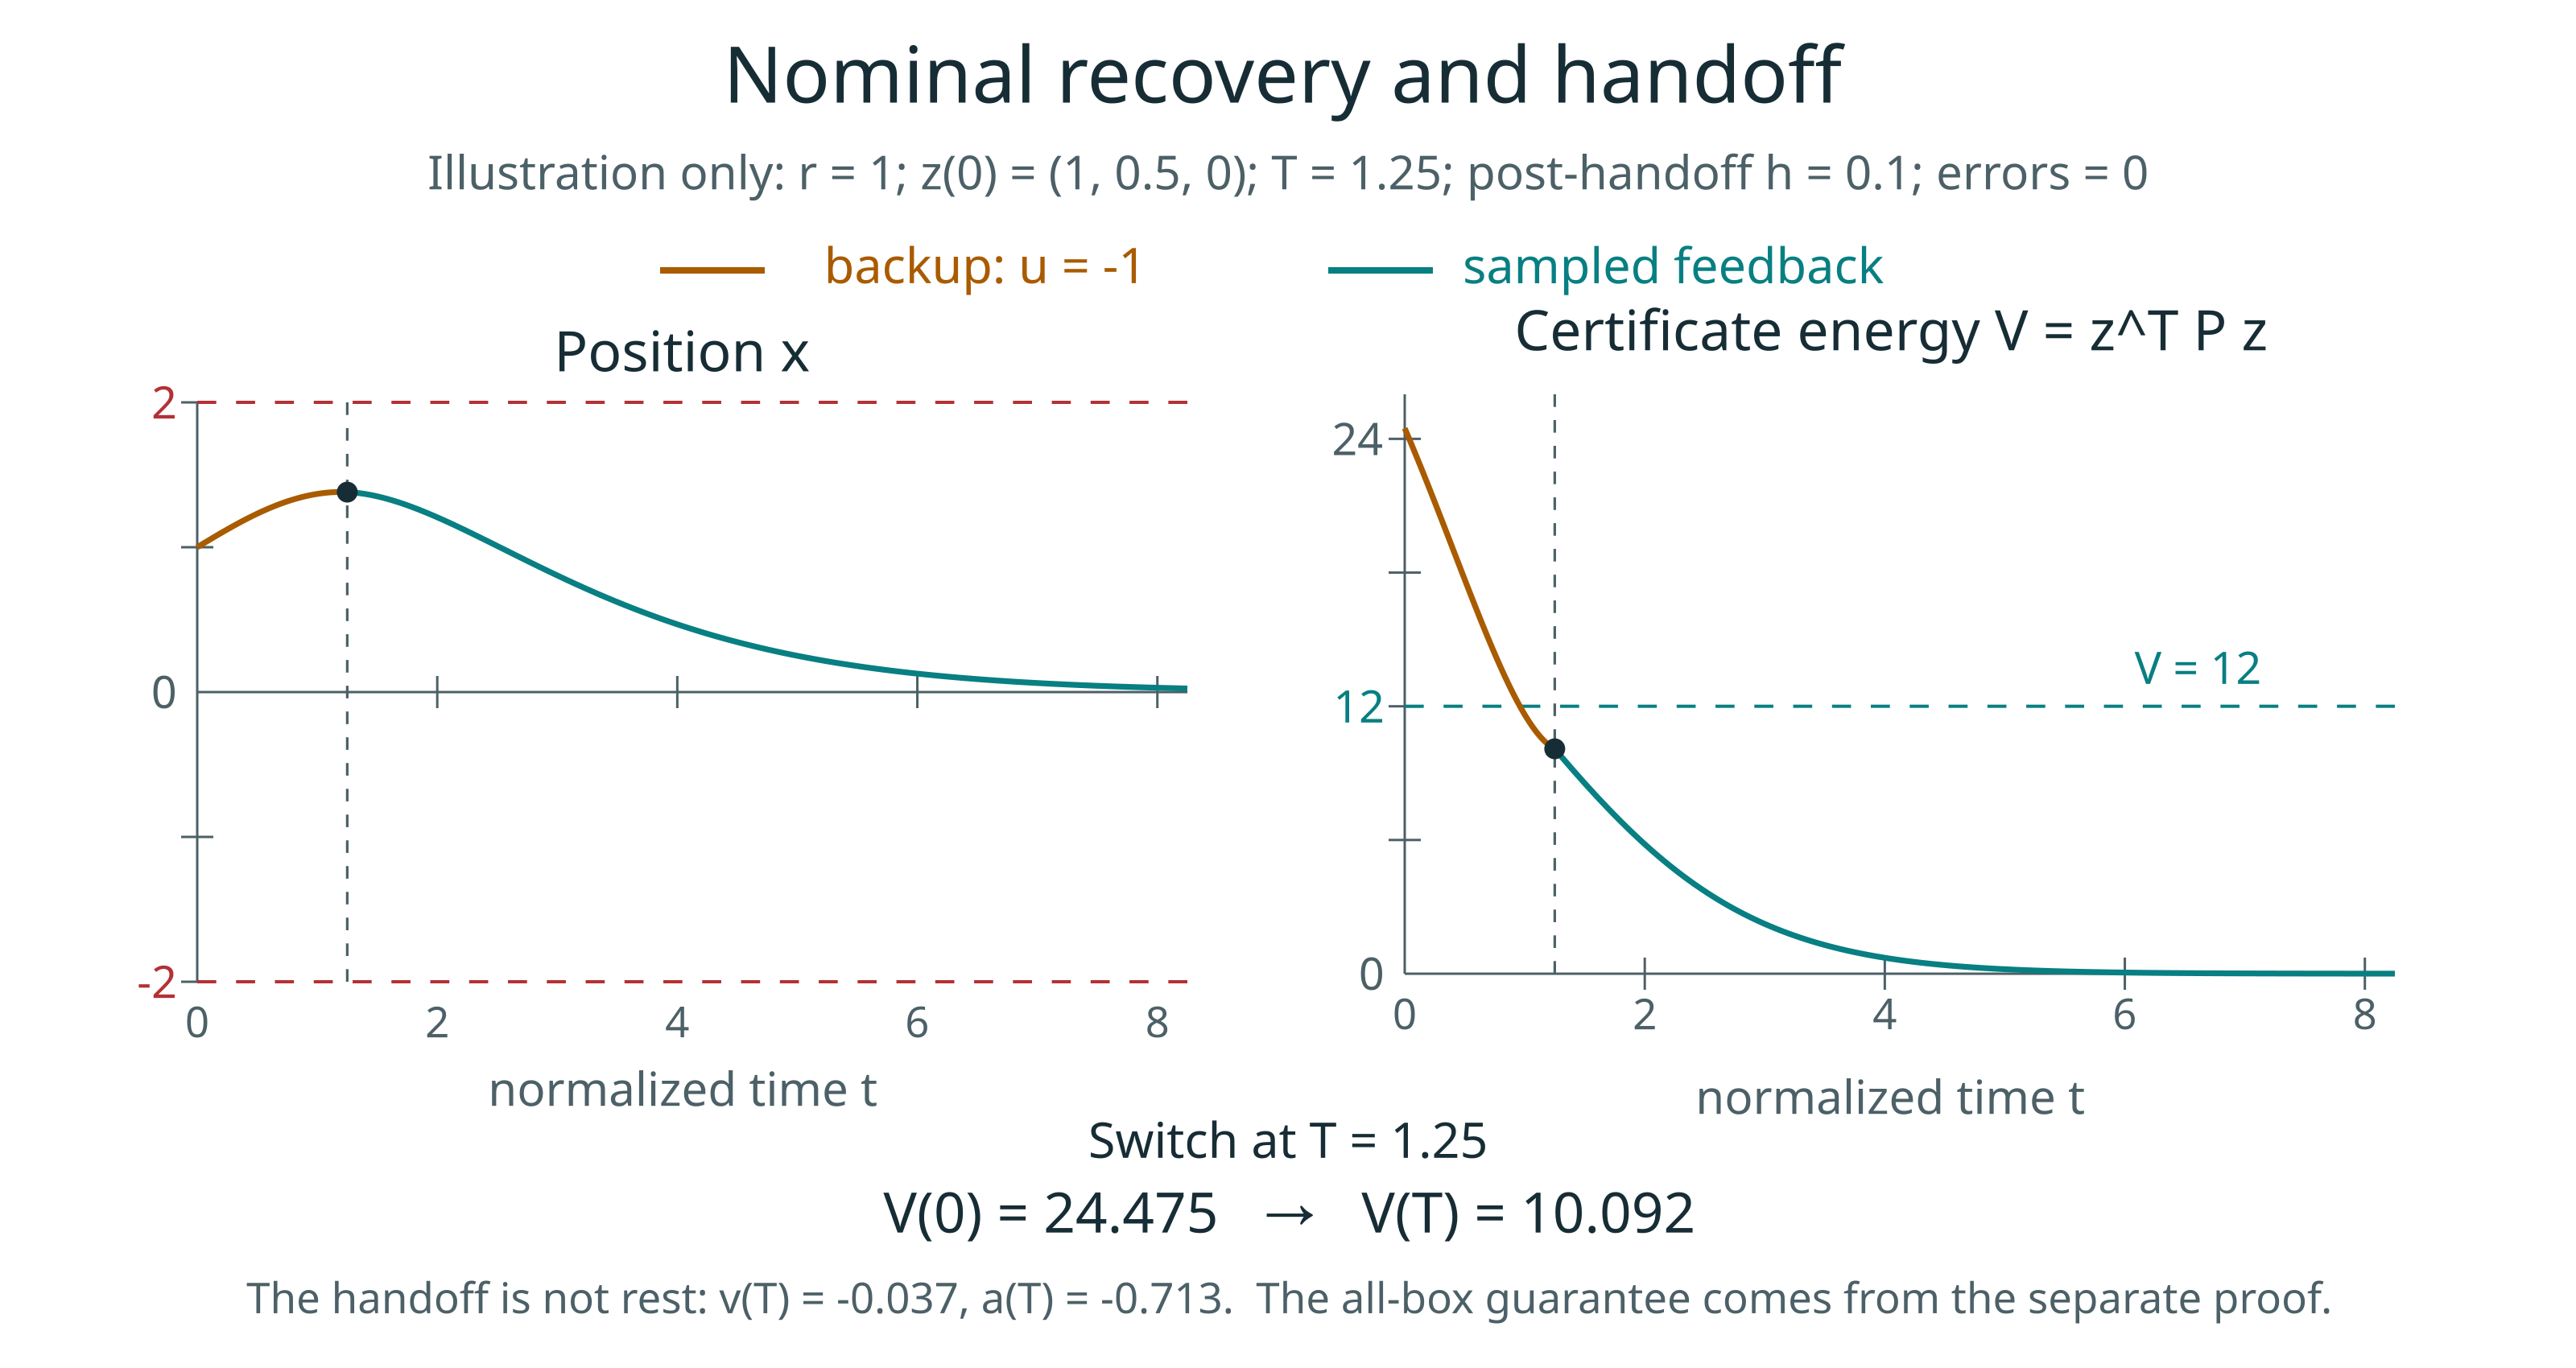
\includegraphics[width=\textwidth]{images/nominal-handoff.png}
\caption{A nominal trajectory from the Manim animation. Here $r=1$, $z_0=(1,1/2,0)$, $T=1.25$, and the later holds have length $0.1$. All errors are zero. The handoff preserves the full state, which is not at rest. The plotted quadratic $V$ is a mathematical certificate, not mechanical energy. This illustration does not prove the whole-box result. The matched interval comparison below uses holds of $0.05$.}
\label{fig:handoff}
\end{figure}

\Needspace{12\baselineskip}
For illustration only, $\tau_0=0.1\,\mathrm{s}$ and $U=2\,\mathrm{m/s^2}$ give:
\begin{center}\small
\begin{tabular}{@{}ll@{}}
\toprule
Quantity & Value\\\midrule
Initial position & $1.98$--$2.02$ cm\\
Initial velocity & $0.098$--$0.102$ m/s\\
Initial acceleration & $-0.02$--$0.02$ m/s$^2$\\
Recovery duration & $125$ ms\\
Position envelope & $\pm4$ cm\\
Maximum later hold & $20$ ms\\
Certified recovery path & $1.6425$--$3.310625$ cm\\\bottomrule
\end{tabular}
\end{center}
These are scaled benchmark values, not measured robot parameters.

\subsection{A possible application and the missing physical evidence}
Figure~\ref{fig:carriage} gives the simplest interpretation: an ideal carriage moves along a rail between two position limits. Its acceleration follows a command with first-order lag. A possible real application is a horizontal stage with an inner acceleration servo. This is an application hypothesis, not a validated model of a particular stage.

The command $u$ is an acceleration reference. It is not automatically motor torque, voltage, or a trajectory acceleration limit. For example, ROS~2 control can forward desired acceleration through a suitable joint interface~\cite{rosaccel}. That interface does not establish the actuator ODE used here. Friction, load changes, delay, flexible modes, and sensor error can require additional states or disturbance terms.

A physical claim needs a selected drive interface and measured model bounds over a stated operating domain. The initial estimation-error set must fit inside the admitted region. The proof must also cover the resulting command errors and timing uncertainty. The exact zero-error prefix is the main current restriction. Figure~\ref{fig:handoff} explains the mathematical mechanism; it cannot supply this missing physical evidence.

\section{Experiments, reproducibility, and contribution limits}
\subsection{A comparison that limits the performance claim}
We compare the recovery policy with direct sampled feedback from the same initial state. There are 24 matched pairs: eight box corners and rates $.9,1,1.1$. Both methods use exact held-flow formulas evaluated in floating point, zero errors, a period of $.1$, and a horizon of 20 normalized time units. Travel extrema are found numerically within held segments; energy is sampled at spacing at most $.005$. None of these numerical measurements is a rigorous upper bound.

\begin{center}\small
\begin{tabular}{@{}lrr@{}}
\toprule
Observed range over 24 runs & Direct feedback & Recovery then feedback\\\midrule
Peak $|x|$ & $1.34229$--$1.42826$ & $1.34013$--$1.42717$\\
Energy at $T$ & $9.19664$--$11.25776$ & $9.60379$--$11.07070$\\
Command total variation & $1.38158$--$1.57972$ & $1.54551$--$1.85423$\\
Observed travel violations & 0 & 0\\\bottomrule
\end{tabular}
\end{center}
Recovery lowers peak travel by only $.00109$--$.00222$ in paired runs. Its terminal energy is better in 13 pairs and worse in 11, and its command total variation is higher in every pair. Direct feedback also enters $\mathcal S$ before $T$ in every tested case. Period checks at $.05$ and $.2$ reach the same qualitative conclusion. The $.05$ case aligns the clocks; at $.1$ and $.2$, the recovery clock restarts at $T$ while the direct clock remains anchored at zero. A finer energy sampling check is included in the artifact.

These tests give no evidence that recovery is necessary or generally better. The Lean proof adds certification from $\mathcal B$, which the old invariant theorem alone does not cover. The next comparison must check the direct-feedback prefix under the same uncertainty and error assumptions.

\subsection{A stronger comparison over the whole box}
We now compare prefixes with a common terminal time $T=5/4$. Both start in $\mathcal B$, use a fixed $r\in[.9,1.1]$, and have zero prefix errors. Direct feedback uses 25 holds of length $1/20$. Recovery holds $u=-1$ until $T$. Both can then start the same robust feedback contract. The complete direct-feedback composition has not yet been checked in Lean.

The direct-feedback prototype divides each initial coordinate into four intervals and the rate into sixteen intervals. The resulting 1,024 closed boxes cover every admitted state and rate. Each arithmetic operation rounds outward on a rational grid with denominator $2^{44}$. Alternating Taylor sums bound the exact held-flow coefficients. The clamp acts on intervals, so the computation includes changes between saturated and unsaturated feedback. An acceleration bound gives position bounds throughout each hold.

For this prototype, the resulting bounds are
\[
\E(z(T))<11.464,\qquad .9887<x(t)<1.4310\quad(0\le t\le T).
\]
These inequalities are outward decimal summaries of exact rational endpoints. All boxes first satisfy the terminal energy test at the sample time $1.2$. The recorded propagation took about $0.58$ seconds. This is Python computation time, not Lean elaboration or kernel replay time.

An independent agent reviewed the interval rules, Taylor bounds, flow identities, and use of convexity. That review found no soundness defect. The full 1,024-cell computation remains outside Lean. The smaller formal pilot below checks one cell through terminal entry. Thus the whole-box result is stronger evidence than tests at selected points, but it is not a second formal safety theorem.

A separate Lean result rules out a tempting shortcut. At $r=1$ and $z_0=(1,1/2,0)$, the request along full braking is
\[
k(t)=t^2/2+3t/2-5/2.
\]
For period $1/10$, the sampled feedback follows full braking through $t=4/5$. It then requests $-49/50$. At that sample, let $E=\exp(-4/5)>0$. The energy is
\[
\E=61323/5000+(997/625)E+(189/50)E^2>12.
\]
The proof uses the sampled recurrence. Thus direct feedback releases full braking while its sampled state is outside the ellipsoid. The invariant theorem cannot start at that sample. A direct-feedback proof must cover the remaining path to a valid entry state. This result does not show unsafe behavior.

\subsection{A fixed family of starting regions}
Before this comparison, we selected four boxes centered at $(1,1/2,0)$. Each coordinate has halfwidth $\lambda/100$, where $\lambda\in\{1,2,4,8\}$. The box volume is $(\lambda/50)^3$. Both methods use the same rate partitions, state partitions, arithmetic, and 25-step prefix. For this comparison, we also split the constant brake into 25 holds. This gives both methods the same propagation structure.

The coarse runs use 1,024 parameter boxes per method and region. One uniform refinement uses 16,384 boxes for every method and region. We made no further changes to seek a winning method. The table gives upper bounds rounded upward. The pass test uses the exact rational bound, with threshold 12.

\begin{center}\small
\begin{tabular}{@{}rrrrr@{}}
\toprule
Box scale & Direct, coarse & Brake, coarse & Direct, refined & Brake, refined\\\midrule
1 & 11.464 & 11.102 & 11.380 & 11.087\\
2 & 12.166 & 11.731 & 12.036 & 11.714\\
4 & 13.678 & 13.155 & 13.467 & 13.131\\
8 & 17.154 & 16.645 & 16.815 & 16.611\\\bottomrule
\end{tabular}
\end{center}

Every path enclosure passes the position test. At scale 2, the brake passes the terminal test and the direct-feedback enclosure does not. This box has eight times the original volume. However, refinement reduces the direct bound from 12.166 to 12.036. Separate corner tests give a largest observed direct energy near 11.933 for this box. The excess may therefore come from the interval method. We have not proved a larger true recovery region or unsafe direct feedback. We have measured a difference in the output of a fixed certificate method. Neither family comparison has yet been checked in Lean.

\subsection{A reusable checker and a formal direct-feedback pilot}
The new checker separates certificate production from acceptance. A producer supplies rational boxes, held-flow coefficient bounds, and an enclosure for each command. Lean proves that accepted one-step containments compose: every admitted initial state remains in its recorded box at each sample. The theorem permits outward rounding between steps. A second theorem connects these discrete states to actual continuous executions of the fixed-rate model. These are endpoint results; they do not by themselves bound the path between samples.

We prove the exponential coefficient bounds on sixteen rate intervals for holds of $1/20$. The concrete pilot checks 25 steps on
\[
 [0.99,0.995]\times[0.49,0.495]\times[-0.01,-0.005],
 \qquad r\in[0.9,0.9125].
\]
This is one of the 1,024 parameter cells in the original comparison. The final interval box implies $V\le12$. The actual-execution theorem therefore gives $V(f(5/4))\le12$, with an existence theorem for such executions. Its contract fixes holds at $0.05$ and errors at zero for all samples, including after $5/4$. It does not yet allow the robust tail in Theorem~1. It also does not establish position safety between the pilot's samples.

This pilot changes the next task. The reusable arithmetic and endpoint composition no longer need to be reproved for each trace. The next proof should bound position over an entire hold from an enclosed starting state and bounded drive. A finite-prefix handoff theorem should then let the prefix restrictions end at sample $N$. These two interfaces would let future certificates reuse the invariant tail. The full covering, certificate-checking cost, and practical value still need evaluation.

\subsection{Verification and trust boundary}
The extension contains seven Lean source modules and 98 audited named theorem declarations. Their fresh source rebuild and individual kernel replay passed; theorem counts describe audit coverage, not research contributions. \code{RecoveryPath} proves the transient bounds and exclusion from $\mathcal S$; \code{TerminalBase} and \code{TerminalCells} prove terminal entry; \code{RecoveryHandoff} proves generic composition and existence; \code{RecoveryBox} discharges the concrete hypotheses; the two physical modules establish the dimensional statements. The certificate producer is untrusted. Its arithmetic assertions are checked in Lean with native evaluation disabled.

The separate \code{DirectSwitch} module contains ten checked declarations. A fresh build, transitive axiom audit, and kernel replay also pass for this module. It proves the sampled release example above. It does not check the Python interval prototype or prove direct-feedback safety.

The seven-module interval-checker extension adds 43 audited named theorems. Its verifier also rebuilds the existing \code{TerminalBase} dependency. Fresh compilation, a transitive axiom audit, and separate kernel replay pass for all eight modules. A deliberately false terminal-energy bound is rejected. This checks the generic endpoint interfaces and the one-cell pilot; it does not certify the full Python comparison. The pilot arithmetic build takes tens of seconds on the local machine. Its manifest separates coefficient regeneration, source compilation, and kernel replay.

The recovery \code{verify.py} script rebuilds its seven modules in an isolated temporary directory. It audits every named theorem's transitive axioms and runs the standalone kernel checker on each module. The separate \code{verify\_switch.py} script applies these checks to \code{DirectSwitch}. Both retain the pinned LeanControls and mathlib artifacts as dependencies. The earlier invariant artifact has its own source replay and certificate-regeneration checks. None of these processes independently bootstraps Lean. Permitted axioms are only \code{propext}, \code{Classical.choice}, and \code{Quot.sound}. Admitted proofs and compiler-trust axioms are excluded. A negative recovery test changes the terminal time while retaining the original formula. The verifier requires that test to fail.

The toolchain is Lean 4.35.0 with mathlib revision \code{56a0058}; the full revision is recorded in the base artifact, and the extension manifest records source hashes, results, log hashes and audit counts. Commands are implemented in \code{verify.py}, with captured output under \code{verification-logs}. From the workspace root, run \texttt{python3 research/adjacent-controls/recovery-proof/verify.py}; the companion README documents the required base project and toolchain paths. The numerical experiment uses Python's standard library, so no numerical solver is needed for this analytic plant.

\subsection{Relation to established methods and remaining gaps}
Backup control barrier functions already define safe regions through a fixed backup flow and compare them with other invariant-set methods \cite{backup}. Disturbance-robust backup CBFs use bounds around nominal flows to address unmodeled disturbances \cite{robustbackup}. Our exact, disturbance-free backup phase is narrower. We do not claim a new recovery architecture or an improved robust-control method.

Formal control-envelope pipelines also predate this artifact. Hellwig et al.\ connect numerical zonotope witnesses to KeYmaera X proofs, including intersample properties \cite{zonotope}. Our candidate contribution is a concrete Lean composition spanning uncertain lag, a long recovery segment, a saturated sampled invariant and continuous actual-execution handoff. A different proof assistant or a new count of theorems is not itself a novelty claim.

The admitted box is small; we do not claim a maximal safe region. The proof assumes an exact switch time and zero brake-phase errors. It does not cover finite-precision code, state estimation, varying lag, friction, or coupled axes. A local explanatory animation accompanies the draft. No hardware test or independent use of the proof interface is reported.

The next publication gate has three parts. First, extend the formal pilot to the full direct-feedback covering, continuous path safety, and a finite-prefix handoff to the robust tail. Second, compare both methods on a fixed family of initial boxes. Record certified volume, certificate size, generation time, elaboration time, and kernel replay time separately. Third, establish external value through independent reuse, comparison with an existing method, or a useful change in supported assumptions. An interval computation that fails to certify a box does not prove that the controller is unsafe. More lemmas alone do not establish a research contribution.

\paragraph{Authorship and assistance.}
This local draft is prepared for Mike and has not been submitted. AI systems assisted exploration, implementation, writing and adversarial review. Full author details, contribution attribution and venue requirements remain for human review.

\begin{thebibliography}{9}\small
\bibitem{backup} Y. Chen, M. Jankovic, M. Santillo, and A. D. Ames.
Backup Control Barrier Functions: Formulation and Comparative Study. 2021.
\url{https://arxiv.org/abs/2104.11332}.
\bibitem{robustbackup} D. E. J. van Wijk, S. Coogan, T. G. Molnar, M. Majji, and K. L. Hobbs.
Disturbance-Robust Backup Control Barrier Functions: Safety Under Uncertain Dynamics.
IEEE Control Systems Letters, 2024.
\url{https://doi.org/10.1109/LCSYS.2024.3514998}.
\bibitem{zonotope} J. Hellwig, L. Sch\"afer, L. Qian, A. Platzer, and M. Althoff.
From Zonotopes to Proof Certificates: A Formal Pipeline for Safe Control Envelopes.
iFM 2025, LNCS 16194, 248--267, 2026.
\url{https://doi.org/10.1007/978-3-032-10794-7_13}.
\bibitem{rosaccel} ROS~2 Control documentation.
Joint trajectory controller, Kilted distribution. Accessed 17 October 2026.
\url{https://control.ros.org/kilted/doc/ros2_controllers/joint_trajectory_controller/doc/userdoc.html}.
\end{thebibliography}
\end{document}
